%%%%%%%%%%%%%%%%%%%%%%%%%%%%%%%%%%%%%%%%%%%%%%%%%%%%%%%%%%%%%%%%%%%%%%%%%%%%%%%%%%%%%%%%%%%%%
%%									Intro    												%
%%%%%%%%%%%%%%%%%%%%%%%%%%%%%%%%%%%%%%%%%%%%%%%%%%%%%%%%%%%%%%%%%%%%%%%%%%%%%%%%%%%%%%%%%%%%%


%%%%%%%%%%%%%%%%%%%%%%%%%%%%%%%%%%%%%%%%%%%%%%%%%%%%%%%%%%%%%%%%%%%%%%%%%%%%%%%%%%%%%%%%%%%%%

\begin{figure}
  \centering
  \reflectbox{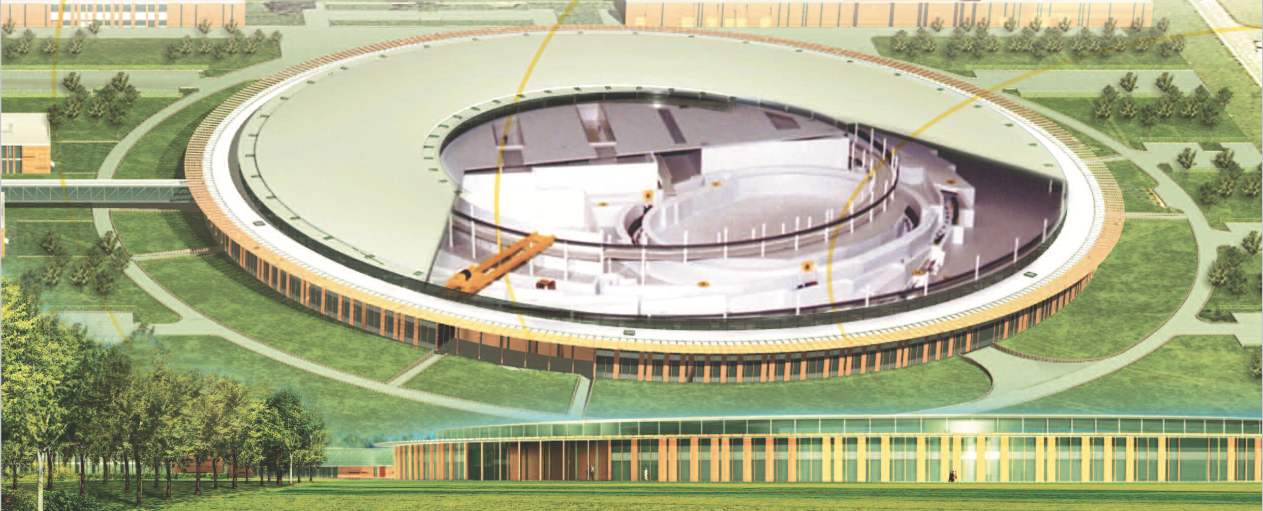
\includegraphics[width=16cm]{Introduction/MaquetteLaboratoire.png}}
  \caption{Maquette du laboratoire Soleil (vue d'artiste)}
\end{figure}
% Début du chapitre
			
\section*{Introduction}



     Mon stage s'est déroulé au synchrotron SOLEIL en région parisienne. 


     %Il a duré cinq jours, du 6 au 10 février chaque jour de 9h à 17h. 

     %Le synchrotron SOLEIL est un immense bâtiment comportant de la très haute technologie. L'élément principal est l'accélérateur d'éléctrons, sur lequel travaille des scientifiques français mais aussi d'autres pays car il n'y a pas beaucoup d'accélérateur de particules dans le monde.
		
     Le synchrotron SOLEIL est un laboratoire de recherche scientifique destiné à l'étude de la matière qu'elle soit vivante ou inerte. Il est un équipé d'un accélérateur d'électrons. Les physiciens exploitent le rayonnement synchrotron émis par les électrons circulant dans l'accélérateur pour fournir des sources de lumière extrêmement brillante.

     Pendant mon stage, j'ai été encadrée par M. Jobert, qui travaille dans le groupe conception et ingénierie en tant qu'ingénieur spécialisé en calcul scientifique. Au cours de mon stage, j'ai aussi découvert l'ensemble des corps de métier qui interviennent pour faire fonctionner le synchrotron.
		
